\chapter{Giới thiệu}
Chương này trình bày tổng quan về bài toán hỗ trợ chẩn đoán bệnh lý trên ảnh X-quang bằng học sâu đa phương thức, 
đặc biệt trong bối cảnh dữ liệu y tế thường có tính phức tạp cao và phụ thuộc mạnh vào kinh nghiệm của bác sĩ 
trong quá trình phân tích. Bên cạnh thông tin hình ảnh, quá trình chẩn đoán thực tế còn yêu cầu kết hợp thêm 
các thông tin lâm sàng và báo cáo y khoa nhằm đưa ra đánh giá toàn diện về tình trạng bệnh nhân. 
Tuy nhiên, việc khai thác hiệu quả đồng thời nhiều nguồn dữ liệu khác nhau vẫn còn là một thách thức lớn 
đối với các hệ thống học sâu hiện nay.

Xuất phát từ thực tế đó, khóa luận hướng đến nghiên cứu và xây dựng một hệ thống học sâu đa phương thức 
kết hợp dữ liệu hình ảnh X-quang và thông tin văn bản lâm sàng nhằm nâng cao hiệu năng phân loại và hỗ trợ chẩn đoán. 
Đồng thời, đề tài cũng khảo sát các phương pháp tinh chỉnh mô hình tiền huấn luyện, 
cơ chế dung hợp dữ liệu nhằm tăng khả năng tận dụng tri thức nền cũng như cải thiện tính minh bạch 
trong quá trình suy luận của mô hình. Kết quả nghiên cứu được kỳ vọng góp phần xây dựng một hệ thống hỗ trợ chẩn đoán 
có độ chính xác cao, khả năng giải thích tốt và tạo tiền đề cho việc ứng dụng các mô hình trí tuệ nhân tạo đa phương thức 
trong lĩnh vực y tế tại Việt Nam.
\label{Chapter1}

\pagebreak

%\section{Lý do chọn đề tài}
\section{Bối cảnh và lý do chọn đề tài}
Hệ xương đóng vai trò rất lớn trong việc nâng đỡ cơ thể, bảo vệ các cơ quan trọng yếu và đảm bảo khả năng vận động của con người. 
Trong những năm gần đây, các bệnh lý và chấn thương xương ngày càng gia tăng do tai nạn giao thông, 
tai nạn lao động, hoạt động thể thao và quá trình lão hóa dân số.
Do đó, chấn thương xương khớp và các bệnh lý về xương là một trong những vấn đề y tế cần được quan tâm đặc biệt nhất, 
đòi hỏi việc chẩn đoán phải được thực hiện nhanh chóng và chính xác. Trong thực hành lâm sàng, 
ảnh X-quang xương là phương tiện chẩn đoán hình ảnh cơ bản, phổ biến và có chi phí thấp, 
cho phép bác sĩ quan sát cấu trúc xương, phát hiện tổn thương và định hướng điều trị ngay từ giai đoạn đầu. 
Tuy nhiên, việc đọc và phân tích ảnh X-quang truyền thống hiện nay phụ thuộc rất lớn vào kinh nghiệm thực tiễn 
và sự tập trung của bác sĩ. Điều này dễ dẫn đến những sai sót không đáng có khi lượng bệnh nhân quá lớn gãy quá tải cho các y bác sĩ. 

Để giải quyết các thách thức này, nhiều nghiên cứu đã ứng dụng các mô hình học sâu vào việc 
giải quyết vấn đề đọc ảnh và đưa ra quyết định dựa trên thông tin trên ảnh. Tuy nhiên, 
các mô hình này vẫn chưa đạt được hiệu quả đủ tốt để đưa vào ứng dụng thực tế như DenseNet và Resnet. 
Một trong các lý do chính đó là các mô hình chỉ mới tiếp cận được các thông tin trong ảnh, 
các y bác sĩ không chỉ dựa vào thông tin thông qua việc đọc ảnh mà còn dựa vào các thông tin từ nhiều nguồn bao gồm: 
thông tin từ bệnh nhân thông qua lời khai và khám lâm sàng sau đó các xét nghiệm cận lâm sàng 
như X-quang kèm với thông tin từ bác sĩ đọc ảnh để bổ trợ, từ đó giúp bác sĩ đưa ra chẩn đoán sơ khởi hay chẩn đoán chính xác. 
Dựa vào thực tế đó, các nghiên cứu hiện nay đang dần chuyển dịch sang hướng tiếp cận đa phương thức nhằm mô phỏng lại 
quá trình chẩn đoán của bác sĩ nhằm nâng cao hiệu năng của hệ thống.

Khác với các mô hình đơn phương thức chỉ xử lý trên một phương thức như ảnh hay văn bản duy nhất, 
các mô hình đa phương thức có thể sử dụng nhiều phương thức và tìm ra sự tương quan giữa các phương thức 
nhằm tạo nên biểu diễn có ý nghĩa hơn từ đó nâng cao hiệu năng của hệ thống. 
Với thực tế lâm sàng hiện nay, các mô hình nghiên cứu tập trung vào kết hợp ngôn ngữ và hình ảnh 
hay còn được gọi là mô hình ngôn ngữ trực quan đang là các mô hình đang nhận được nhiều sự chú ý, 
tiêu biểu có thể nhắc đến là MedCLIP \cite{MedCLIP}, BioMedCLIP \cite{BiomedCLIP} hay BioViL \cite{BioViL}. 
Tuy nhiên, các mô hình này vẫn còn tồn tại nhiều hạn chế khi áp dụng vào thực tế lâm sàng, 
như sự khác biệt về đặc trưng giữa dữ liệu hình ảnh và dữ liệu văn bản, 
dữ liệu y tế thực tế thu thập được thường có số lượng hạn chế và mất cân bằng giữa các lớp bệnh, 
yêu cầu đặc biệt về thiết kế mô hình để tận dụng tối đa thông tin có sẵn và phải có khả năng.

Xuất phát từ những vấn đề trên, đề tài lựa chọn nghiên cứu xây dựng một hệ thống phân loại ảnh X-quang xương đa phương thức 
kết hợp đồng thời thông tin từ ảnh và văn bản nhằm khai thác ưu điểm của cả hai nguồn dữ liệu, 
và mở rộng hơn là bài toán phân loại đa nhãn nhằm phản ánh thực tế lâm sàng, 
khi một bệnh nhân có thể đồng thời mắc nhiều tổn thương hoặc nhiều bệnh lý xương. 
Đồng thời, đề tài nghiên cứu các kỹ thuật thích nghi miền, 
học biểu diễn đa phương thức và học phân loại dựa trên mạng nguyên mẫu (prototipical network) 
nhằm nâng cao khả năng tổng quát của mô hình trong điều kiện 
dữ liệu y tế hạn chế, dữ liệu mất cân bằng và hướng tới khả năng nhận biết các trường hợp nằm ngoài phân phối dữ liệu huấn luyện. 
Kết quả nghiên cứu kỳ vọng sẽ góp phần nâng cao hiệu quả của các hệ thống hỗ trợ chẩn đoán bệnh lý xương và tạo tiền đề cho việc 
ứng dụng các mô hình thị giác–ngôn ngữ trong phân tích ảnh y khoa.

\section{Động lực nghiên cứu}
\subsection{Vị trí của hệ thống phân loại khi áp dụng trong quy trình chẩn đoán thực tế}

Trong thực hành lâm sàng, quá trình chẩn đoán bệnh lý xương thường bao gồm nhiều bước, 
từ khám lâm sàng, chỉ định chụp X-quang, phân tích hình ảnh, kết hợp với các thông tin bệnh án và đưa ra chẩn đoán xác định. 

Sau khi ảnh X-quang được ghi nhận, bác sĩ chẩn đoán hình ảnh sẽ đánh giá các đặc điểm bất thường như vị trí tổn thương, 
hình thái gãy xương, dấu hiệu khối u hoặc các biến đổi bệnh lý khác. Đồng thời, 
bác sĩ cũng tham khảo các thông tin lâm sàng như triệu chứng, tiền sử bệnh, 
ngữ cảnh diễn biến chấn thương và các kết quả xét nghiệm để đưa ra kết quả đọc ảnh trước khi bác sĩ chính đưa ra chẩn đoán cuối cùng. 

Hệ thống được đề xuất trong luận văn được thiết kế nhằm hỗ trợ bác sĩ chính ở giai đoạn phân tích ảnh X-quang. 
Cụ thể, hệ thống sử dụng đồng thời ảnh X-quang và dữ liệu văn bản (bao gồm các thông tin lâm sàng) 
để dự đoán một nhiều nhãn bệnh lý có thể xuất hiện trên cùng một bệnh nhân. 
Việc khai thác đồng thời hai nguồn dữ liệu giúp mô hình tận dụng các thông tin bổ sung mà chỉ riêng ảnh 
hoặc văn bản khó có thể biểu diễn đầy đủ.

Khác với các hệ thống chỉ thực hiện phân loại đơn nhãn, hệ thống trong luận văn được xây dựng cho bài toán phân loại đa nhãn 
nhằm phản ánh tốt hơn thực tế lâm sàng, khi một bệnh nhân có thể đồng thời mắc nhiều tổn thương hoặc nhiều bệnh lý xương. 
Bên cạnh đó, hệ thống còn được định hướng tích hợp cơ chế phát hiện dữ liệu ngoài phân phối (Out-of-Distribution - OOD) 
nhằm cảnh báo khi gặp các trường hợp nằm ngoài phạm vi dữ liệu đã được huấn luyện. 
Trong các tình huống này, hệ thống sẽ không đưa ra dự đoán với độ tin cậy cao mà chuyển quyền quyết định cho bác sĩ chuyên môn, 
góp phần nâng cao tính an toàn khi ứng dụng trong thực tế.

Cần lưu ý rằng hệ thống được đề xuất không thay thế vai trò của bác sĩ mà đóng vai trò là công cụ hỗ trợ ra quyết định. 
Các kết quả dự đoán của mô hình cung cấp thông tin tham khảo giúp bác sĩ 
rút ngắn thời gian đọc phim, giảm nguy cơ bỏ sót tổn thương và nâng cao hiệu quả chẩn đoán, 
đặc biệt trong các cơ sở y tế có khối lượng bệnh nhân lớn hoặc thiếu bác sĩ chuyên khoa.

\subsection{Ý nghĩa khoa học của đề tài}

Đề tài góp phần làm rõ vai trò của dữ liệu văn bản lâm sàng trong bài toán phân loại đa nhãn ảnh X-quang xương 
theo hướng đa phương thức. Thông qua việc khai thác đồng thời thông tin từ ảnh X-quang và văn bản, 
nghiên cứu đánh giá mức độ đóng góp của từng phương thức dữ liệu, từ đó làm cơ sở cho việc xây dựng các hệ thống 
hỗ trợ chẩn đoán có khả năng tận dụng hiệu quả nguồn dữ liệu y tế đa dạng trong thực tế.

Trọng tâm của nghiên cứu là khám phá và ứng dụng các kiến trúc mạng ngôn ngữ trực quan, cụ thể là BiomedCLIP \cite{BiomedCLIP}, 
nhằm tận dụng tri thức đã học từ các mô hình tiền huấn luyện trên dữ liệu y tế đa phương thức. 
Cách tiếp cận này góp phần mở rộng khả năng ứng dụng của các mô hình ngôn ngữ trực quan 
trong các bài toán y khoa có dữ liệu chuyên biệt.

Đồng thời, đề tài đi sâu vào việc phát triển hệ thống có khả năng phân loại dưới điều kiện dữ liệu hạn chế, 
mất cân bằng và có sự xuất hiện của các trường hợp ngoài phân phối, 
khi dữ liệu huấn luyện được đánh nhãn đầy đủ không khả dụng nhiều, việc bảo toàn tri thức gốc là một thách thức lớn 
và cũng như đảm bảo mô hình không phân nhãn cho một ca bệnh mới chưa từng xuất hiện trong dữ liệu của bệnh viện.

Đề tài góp phần giải thích kết quả phân loại bằng cách trực quan hóa các vùng ảnh X-quang mà mô hình tập trung khi đưa ra dự đoán, 
giúp bác sĩ hiểu được cơ sở ra quyết định của mô hình.

\subsection{Ý nghĩa thực tiễn của đề tài}

Đề tài xây dựng bộ dữ liệu ảnh X-quang xương được thu thập từ dữ liệu thực tế tại Bệnh viện Chấn thương 
Chỉnh hình Thành phố Hồ Chí Minh, đồng thời tiến hành chuẩn hóa, tinh lọc và xây dựng hệ thống nhãn phục vụ 
cho bài toán phân loại đa nhãn. Bộ dữ liệu này có giá trị tham khảo cho các nghiên cứu tiếp theo về phân tích 
ảnh X-quang xương và phát triển các mô hình trí tuệ nhân tạo trong lĩnh vực chẩn đoán hình ảnh ở thực tế.

Bên cạnh việc đưa ra một kết quả phân tích ảnh mang tính chất hỗ trợ chẩn đoán, 
mô hình còn được thiết kế để cung cấp các bản đồ nhiệt trực quan hóa trên ảnh X-quang, 
giúp bác sĩ hiểu được cơ sở ra quyết định của mô hình, 
từ đó nâng cao tính minh bạch và độ tin cậy khi triển khai trong thực tế lâm sàng.

Hệ thống được đề xuất hướng đến giải quyết các thách thức thường gặp trong dữ liệu thực tế ở lĩnh vực y tế nước nhà 
như số lượng mẫu gán nhãn hạn chế, mất cân bằng giữa các lớp bệnh khi một ca bệnh có tỉ trọng cao hơn 
và sự xuất hiện của các trường hợp ngoài phân phối khi gặp một căn bệnh mới. 
Việc xây dựng hệ thống đối phó được với các thách thức này giúp nâng cao khả năng tổng quát của mô hình, 
tăng độ tin cậy khi triển khai trong môi trường lâm sàng nước ta với dữ liệu y tế phục vụ huấn luyện còn hạn chế, 
cũng như giúp phát hiện một ca bệnh chưa từng xuất hiện trong dữ liệu của bệnh viện.

Bên cạnh với đối phó về thiếu hụt dữ liệu để đáp ứng thực tế, đề tài phát triển hệ thống hỗ trợ phân loại 
bệnh lý xương từ ảnh X-quang theo quy trình gần với thực tế lâm sàng. 
Trong quá trình huấn luyện, mô hình được khai thác thông tin từ báo cáo phân tích ảnh nhằm học được mối liên hệ giữa hình ảnh 
và tri thức chuyên môn. Khi đưa vào sử dụng, hệ thống chỉ yêu cầu ảnh X-quang kết hợp với các thông tin lâm sàng ban đầu 
như triệu chứng, cơ chế chấn thương hoặc chẩn đoán sơ bộ của bác sĩ để đưa ra dự đoán. 
Cách tiếp cận này mô phỏng quy trình ra quyết định của bác sĩ trong thực tế, góp phần nâng cao khả năng ứng dụng của 
hệ thống trong hỗ trợ chẩn đoán và giảm phụ thuộc vào các báo cáo chẩn đoán chuyên sâu vốn chưa có tại thời điểm tiếp nhận bệnh nhân.

\section{Định nghĩa các khái niệm}
Nhằm đảm bảo sự thống nhất trong quá trình nghiên cứu và trình bày, một số khái niệm cơ bản được định nghĩa như sau:
\subsection{Thông tin lâm sàng}
Thông tin lâm sàng là những dữ liệu thu thập trực tiếp qua quá trình bác sĩ thăm khám người bệnh, 
bao gồm việc khai thác bệnh sử và khám thực thể (nhìn, sờ, gõ, nghe) \cite{Dorland2011}. 
Dữ liệu này mang tính chất định hướng ban đầu, giúp bác sĩ khoanh vùng tổn thương và đưa ra các quyết định 
chỉ định thăm khám chuyên sâu tiếp theo \cite{Bickley2020_Bates}.
\begin{figure}[H]
    \centering
    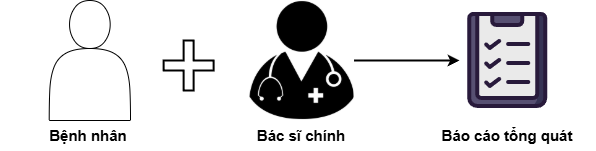
\includegraphics[width=0.8\linewidth]{images/ClinicalSource.png}
    \caption{Nguồn thông tin lâm sàng bao gồm khai thác bệnh sử và khám thực thể}
    \label{fig:clinical_source}
\end{figure}

\subsection{Thông tin cận lâm sàng}
Thông tin cận lâm sàng là các dữ liệu khách quan thu được từ việc áp dụng các trang thiết bị và kỹ thuật y khoa hiện đại 
(như hình ảnh X-quang, cắt lớp, hay xét nghiệm sinh hóa) \cite{Dorland2011}. Nếu lâm sàng dùng để định hướng, 
thì cận lâm sàng cung cấp bằng chứng xác thực từ bên trong cơ thể để chẩn đoán chính xác bệnh lý.
\begin{figure}[H]
    \centering
    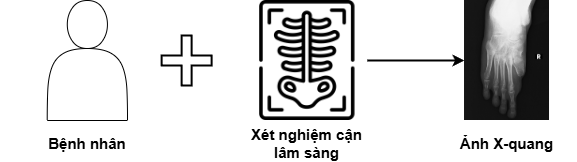
\includegraphics[width=0.8\linewidth]{images/XraySource.png}
    \caption{Nguồn thông tin cận lâm sàng từ hình ảnh X-quang}
    \label{fig:xray_source}
\end{figure}

Ngoài ra, thông tin cận lâm sàng còn bao gồm các báo cáo đọc ảnh của bác sĩ đọc ảnh, 
đây là những dữ liệu văn bản được trích xuất từ quá trình phân tích hình ảnh y tế, 
cung cấp các nhận định chuyên môn về tình trạng bệnh nhân dựa trên hình ảnh thu được \cite{Bickley2020_Bates}.
\begin{figure}[H]
    \centering
    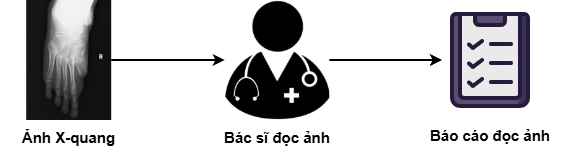
\includegraphics[width=0.8\linewidth]{images/XrayReportSource.png}
    \caption{Nguồn thông tin từ báo cáo đọc ảnh X-quang}
    \label{fig:xray_report_source}
\end{figure}

\section{Giới thiệu bài toán}

Bài toán được nghiên cứu trong đề tài là bài toán phân loại đa nhãn ảnh X-quang sử dụng học sâu đa phương thức. 
Mục tiêu của hệ thống là dự đoán các loại bệnh hoặc tổn thương dựa trên đồng thời dữ liệu hình ảnh X-quang 
và thông tin văn bản lâm sàng liên quan.

\begin{itemize}
  \item \textbf{Đầu vào (Input):} Hệ thống nhận vào các nguồn dữ liệu sau:

  \begin{itemize}
    \item Ảnh X-quang của bệnh nhân:
    \[
        x^{img} \in \mathrm{R}^{H \times W \times C}
    \]
    trong đó:
    \begin{itemize}
        \item $H, W$: chiều cao và chiều rộng ảnh,
        \item $C$: số kênh màu của ảnh.
    \end{itemize}

    \pagebreak

    \item Thông tin văn bản lâm sàng gồm các báo cáo đọc ảnh của bác sĩ đọc ảnh, lời khai bệnh nhân và lịch sử bệnh lý được biểu diễn dưới dạng chuỗi token:
    \[
        x^{txt} = \{w_1, w_2, ..., w_T\}
    \]
    trong đó:
    \begin{itemize}
        \item $w_t$: token thứ $t$,
        \item $T$: số lượng token trong văn bản.
    \end{itemize}

    \item Tập nhãn được định nghĩa trước:
    \[
        \mathcal{Y} = \{y_1, y_2, ..., y_K\}
    \]
    với $K$ là số lớp bệnh cần phân loại.
  \end{itemize}

  \item \textbf{Đầu ra (Output):} Hệ thống sinh ra:

  \begin{itemize}
    \item Các nhãn dự đoán cuối cùng, được sắp xếp theo thứ tự:
    \[
        y^{*} = \arg\max_{k \in \{1,...,K\}} \hat{y}_k
    \]

    \item Bản đồ nhiệt trực quan hóa trên ảnh nhằm giải thích dự đoán của mô hình
  \end{itemize}
\end{itemize}

\subsection{Các thách thức trong bài toán}

Mặc dù các mô hình học sâu đa phương thức đã đạt được nhiều kết quả tích cực, bài toán vẫn tồn tại nhiều thách thức cần được giải quyết:

\begin{itemize}
    \item Tồn tại sự chênh lệch lớn giữa các bộ dữ liệu đa phương thức hiện có (thường là cặp ảnh X-quang và báo cáo đọc ảnh X-quang) 
    so với luồng công việc thực tế lâm sàng (bao gồm ảnh chụp X-quang kết hợp với báo cáo tổng quát), làm hạn chế khả năng ứng dụng trực tiếp của các mô hình.
    \item Sự khác biệt về đặc trưng giữa dữ liệu hình ảnh và dữ liệu văn bản gây khó khăn cho quá trình học biểu diễn chung, yêu cầu một cơ chế dung hợp hiệu quả.
    \item Dữ liệu y tế thường có số lượng hạn chế và mất cân bằng giữa các lớp bệnh, đặt ra yêu cầu đặc biệt về thiết kế mô hình để tận dụng tối đa thông tin có sẵn.
    \item Trong thực tế lâm sàng, luôn có tỉ lệ xuất hiện những loại bệnh mới nằm ngoài dữ liệu huấn luyện, đặt ra yêu cầu về khả năng tổng quát hóa và thích ứng của mô hình.
    \item Khả năng giải thích của mô hình vẫn còn hạn chế, gây khó khăn cho việc triển khai trong thực tế lâm sàng.
\end{itemize}

\subsection{Các hướng tiếp cận hiện có}
Các nghiên cứu hiện nay chủ yếu tiếp cận bài toán theo ba hướng chính:

\begin{itemize}
    \item Các phương pháp đa phương thức kết hợp dữ liệu hình ảnh và văn bản thông qua các chiến lược dung hợp đặc trưng nhằm khai thác mối tương quan giữa các phương thức dữ liệu.
    \item Các mô hình ngôn ngữ thị giác quy mô lớn được huấn luyện trước trên dữ liệu đa phương thức nhằm học biểu diễn chung giữa ảnh và văn bản.
    \item Các mô hình ngôn ngữ lớn đa phương thức được huấn luyện trên nhiều tác vụ khác nhau nhằm tăng khả năng suy luận, hiểu ngữ cảnh và hỗ trợ ra quyết định trong các bài toán y tế phức tạp.
\end{itemize}

Tuy đã đạt được nhiều kết quả khả quan, các nghiên cứu hiện nay phần lớn vẫn tiếp cận vấn đề một cách rời rạc. Chúng thường chỉ tập trung giải quyết riêng lẻ từng thách thức như tiền huấn luyện trên dữ liệu y khoa, học với ít mẫu (few-shot learning) hay phát hiện dữ liệu ngoài phân phối (out-of-distribution detection), mà thiếu đi một khuôn khổ thống nhất. Đáng chú ý nhất, các phương pháp này tồn tại một khoảng trống lớn so với thực tiễn: chúng gần như chỉ phụ thuộc vào cặp dữ liệu ảnh X-quang và báo cáo đọc ảnh X-quang. Việc bỏ qua các báo cáo lâm sàng tổng quát (nguồn thông tin bối cảnh mang tính quyết định) làm giảm đáng kể tính ứng dụng của mô hình. Hơn nữa, việc khai thác mối tương quan ngữ nghĩa đa phương thức giữa hình ảnh và văn bản vẫn chưa đạt hiệu quả tối ưu, kéo theo những hạn chế về khả năng giải thích quá trình suy luận và ra quyết định.

% \section{Mục tiêu nghiên cứu}
% Đề tài hướng đến việc nghiên cứu và xây dựng một hệ thống học sâu đa phương thức phục vụ hỗ trợ phân loại ảnh X-quang kết hợp với thông tin lâm sàng. Hệ thống được kỳ vọng có khả năng khai thác hiệu quả mối tương quan giữa dữ liệu hình ảnh và báo cáo lâm sàng nhằm nâng cao hiệu năng chẩn đoán so với các mô hình đơn phương thức truyền thống.

% Các mục tiêu cụ thể của đề tài bao gồm:
% \begin{itemize}
%   \item Khảo sát và phân tích các phương pháp học sâu đa phương thức trong bài toán phân loại ảnh y tế.
%   \item Nghiên cứu các chiến lược dung hợp dữ liệu hình ảnh và văn bản nhằm khai thác tối đa thông tin đa nguồn.
%   \item Nghiên cứu các cơ chế phát hiện dữ liệu ngoài phân phối (out-of-distribution detection) nhằm tăng khả năng tổng quát hóa và độ tin cậy của mô hình trong môi trường lâm sàng thực tế.
%   \item Khảo sát các phương pháp tinh chỉnh tham số hiệu quả cho các mô hình tiền huấn luyện nhằm giảm chi phí huấn luyện và tận dụng tri thức đã có.
%   \item Xây dựng cơ chế giải thích giúp trực quan hóa cơ sở đưa ra quyết định của mô hình.
%   \item Đánh giá hiệu năng và khả năng tổng quát hóa của mô hình trên các bộ dữ liệu công khai và dữ liệu nội bộ.
% \end{itemize}

\section{Đối tượng và phạm vi nghiên cứu}
\subsection{Đối tượng nghiên cứu}
Đối tượng nghiên cứu của đề tài là các mô hình học sâu đa phương thức sử dụng đồng thời dữ liệu hình ảnh và văn bản trong bài toán phân loại ảnh X-quang. Nghiên cứu tập trung vào các thành phần chính của một hệ thống đa phương thức bao gồm bộ mã hóa ảnh, bộ mã hóa văn bản, mô-đun dung hợp dữ liệu và bộ phân loại.

Ngoài ra, đề tài cũng khảo sát các phương pháp tinh chỉnh tham số hiệu quả cho các mô hình đã được huấn luyện trước nhằm tận dụng tri thức nền và cải thiện hiệu năng trên tác vụ đích.

\begin{figure}[H]
    \centering
    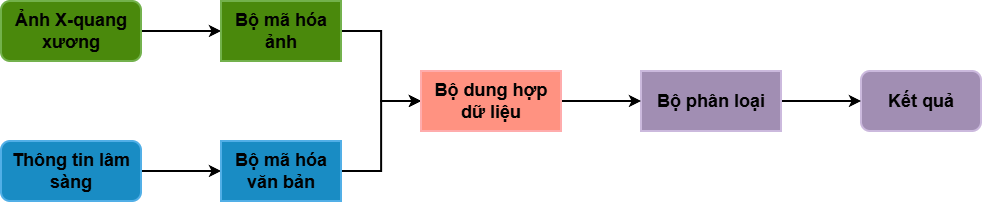
\includegraphics[width=1\linewidth]{images/Pipeline.png}
    \caption{Khung chương trình tổng quát cho một hệ thống phân loại ảnh sử dụng học sâu đa phương thức}
    \label{fig:pipeline}
\end{figure}

\subsection{Phạm vi nghiên cứu}
Đề tài tập trung nghiên cứu các bài toán phân loại trên ảnh X-quang kết hợp với thông tin văn bản lâm sàng. 
Dữ liệu văn bản được sử dụng bao gồm báo cáo đọc ảnh, thông tin lâm sàng.

Hệ thống được sử dụng với vai trò là một công cụ hỗ trợ chẩn đoán, không thay thế vai trò của bác sĩ trong quá trình ra quyết định.

Nghiên cứu chủ yếu sử dụng các bộ dữ liệu cặp ảnh – văn bản đã được công bố công khai cùng với bộ dữ liệu 
nội bộ được cung cấp thông qua hợp tác với bệnh viện tại Thành phố Hồ Chí Minh. 
Các bộ dữ liệu này được sử dụng nhằm đánh giá hiệu năng, khả năng tổng quát hóa và tính hiệu quả của mô hình đề xuất 
thông qua các độ đo phổ biến trong bài toán phân loại.

Đề tài không tập trung vào các bài toán khác như phát hiện đối tượng, phân đoạn ảnh hay sinh báo cáo y khoa tự động.

\section{Bố cục luận văn}
Khóa luận được trình bày một cách hệ thống và logic qua 5 chương, dẫn dắt người đọc từ tổng quan lý thuyết đến thực nghiệm chi tiết và kết luận:

\textbf{Chương 1: Giới thiệu.} Chương này cung cấp cái nhìn tổng quan về bối cảnh nghiên cứu, xác định rõ vấn đề cần giải quyết, mục tiêu, phương pháp tiếp cận và những đóng góp chính của đề tài. Đây là phần nền tảng định hướng cho toàn bộ nội dung khóa luận.

\textbf{Chương 2: Các công trình nghiên cứu liên quan.} Chương này tập trung hệ thống hóa các hướng tiếp cận đã được mô tả ở trên, làm tiền đề cho việc xây dựng giải pháp của khóa luận. Trọng tâm của chương là việc phân tích các kiến trúc mô hình thị giác - ngôn ngữ tiên tiến cùng các chiến lược dung hợp đặc trưng đa phương thức. Bên cạnh đó, các kỹ thuật tinh chỉnh tối ưu và phương pháp nhận diện dữ liệu ngoài phân phối cũng được xem xét toàn diện, từ đó thiết lập cơ sở lý thuyết vững chắc và định vị rõ ràng hướng giải quyết của đề tài so với các công trình đi trước.

\textbf{Chương 3: Phương pháp đề xuất.} Đây là chương trọng tâm mô tả chi tiết quy trình xây dựng hệ thống. Tại đây, nhóm sẽ trình bày cụ thể về kiến trúc mô hình Med-VLM được lựa chọn, quy trình xử lý dữ liệu đầu vào (cả ảnh và văn bản), thiết kế các hàm mất mát (loss functions), và chiến lược huấn luyện mô hình (training strategy). Các sơ đồ khối và thuật toán sẽ được mô tả chi tiết để minh họa cho giải pháp.

\textbf{Chương 4: Thực nghiệm và Kết quả.} Chương này trình bày về bộ dữ liệu được sử dụng, thiết lập môi trường thực nghiệm và các chỉ số đánh giá (metrics) như Accuracy, F1-Score, AUC-ROC. Kết quả thực nghiệm sẽ được phân tích sâu, so sánh đối chiếu với các phương pháp khác để làm rõ ưu nhược điểm của mô hình đề xuất. Các phân tích sai số (error analysis) cũng được thực hiện để hiểu rõ hành vi của mô hình.

\textbf{Chương 5: Kết luận và Hướng phát triển.} Chương cuối cùng tổng kết lại những kết quả đạt được so với mục tiêu ban đầu, nhìn nhận thẳng thắn những hạn chế còn tồn tại của hệ thống và đề xuất các hướng nghiên cứu tiếp theo để hoàn thiện và mở rộng ứng dụng trong tương lai.